
\documentclass[refman]{article}
\usepackage[utf8]{inputenc}
\usepackage[english]{babel}


%

\usepackage{colortbl}
\usepackage{epigraph}
\usepackage{fancyhdr}
\usepackage{graphicx}
\usepackage{hhline}
\usepackage{biblatex}

\usepackage[procnames]{listings}
\usepackage{longtable}
\usepackage{tikz}
\usepackage{subcaption}
\usepackage{xcolor}
\usepackage{wrapfig}
\usepackage[nottoc,numbib]{tocbibind}
%
%\usepackage[T1]{fontenc}
\usepackage{lmodern}

\usepackage{amsfonts}
\usepackage{amsmath}
\usepackage{amsthm}
\usepackage{mathtools}

\usepackage{geometry}
 \geometry{
 a4paper,
 left=30mm,
 top=30mm,
 }
\pagestyle{fancy}

\newcommand{\idx}{\text{idx}}

\DeclarePairedDelimiter\ceil{\lceil}{\rceil}
\DeclarePairedDelimiter\floor{\lfloor}{\rfloor}

\theoremstyle{definition}
\newtheorem*{formula}{Formula}

\usepackage[document]{ragged2e}

\begin{document}

\section{Introduction}

Previously \cite{xxx}, we discussed the numerical approach to the Poisson's equation. In essence, if we denote the dimension with \(d\), then the domain \(\Omega := [0, 1]^d\) is discretized into \(N^d\) points and the problem is reduced to a linear equation that is

\begin{align*}
	A^{(d)} u = b
\end{align*}

where \(A^{(d)}\) is the matrix which has a sparse structure defined in the last protocol. We will now explore numerical methods to solve the linear equation above.

For this, consider the function

\begin{align*}
	u(x) := \prod_{l=1}^d x_l \sin (\kappa \pi x_l)
\end{align*}

and since the Poisson's equation we want to solve is the following

\begin{align*}
	f(x) = - \Delta u(x) = -\sum_{l = 1}^d \frac{\partial^2 u}{\partial x_l^2} (x)
\end{align*}

we have

\begin{align*}
	f_{d=1} (x_1) =& \kappa \pi \left( \kappa \pi x_1 \sin ( \kappa \pi x ) - 2 \cos( \kappa \pi x_1) \right) \\
%	
	f_{d=2} (x_1, x_2) =& \kappa \pi x_2 \sin( \kappa \pi x_2) \left(  \kappa \pi x_1 \sin(\kappa \pi x_1) - 2 \cos ( \kappa \pi x_1) \right) + \\ 
	& \kappa \pi x_1 \sin( \kappa \pi x_1) \left(  \kappa \pi x_2 \sin(\kappa \pi x_2) - 2 \cos ( \kappa \pi x_2) \right) \\
%
	f_{d=3} (x_1, x_2, x_3) =& \kappa \pi x_2 \sin( \kappa \pi x_2) \kappa \pi x_3 \sin(\kappa \pi x_3)  \left(  \kappa \pi x_1 \sin(\kappa \pi x_1) - 2 \cos ( \kappa \pi x_1) \right) + \\
	& \kappa \pi x_1 \sin( \kappa \pi x_1) \kappa \pi x_3 \sin(\kappa \pi x_3)  \left(  \kappa \pi x_2 \sin(\kappa \pi x_2) - 2 \cos ( \kappa \pi x_2) \right) + \\
	& \kappa \pi x_1 \sin( \kappa \pi x_1) \kappa \pi x_2 \sin(\kappa \pi x_2)  \left(  \kappa \pi x_3 \sin(\kappa \pi x_3) - 2 \cos ( \kappa \pi x_3) \right) \text{.}
\end{align*}

We want to now solve the given linear equation for \(u\) (we will denote the numerical solution with \(\hat{u}\)) for each dimension and compare it with the original \(u\). To do this, we first apply the LU-decomposition to \(A^{(d)}\) and multiply the inverse of \(L\) and \(U\) with \(b\) to get \(b\).

\section{User Manual}

\section{Error and Condition}

We have drawn the plot of the absolute difference of \(u\) and \(\hat{u}\) for \(d = 1, 2, 3\) with the number of grid points on an axis \(N\) as the variable (see figure \ref{fig:plot_error}).

\begin{figure}[h]
	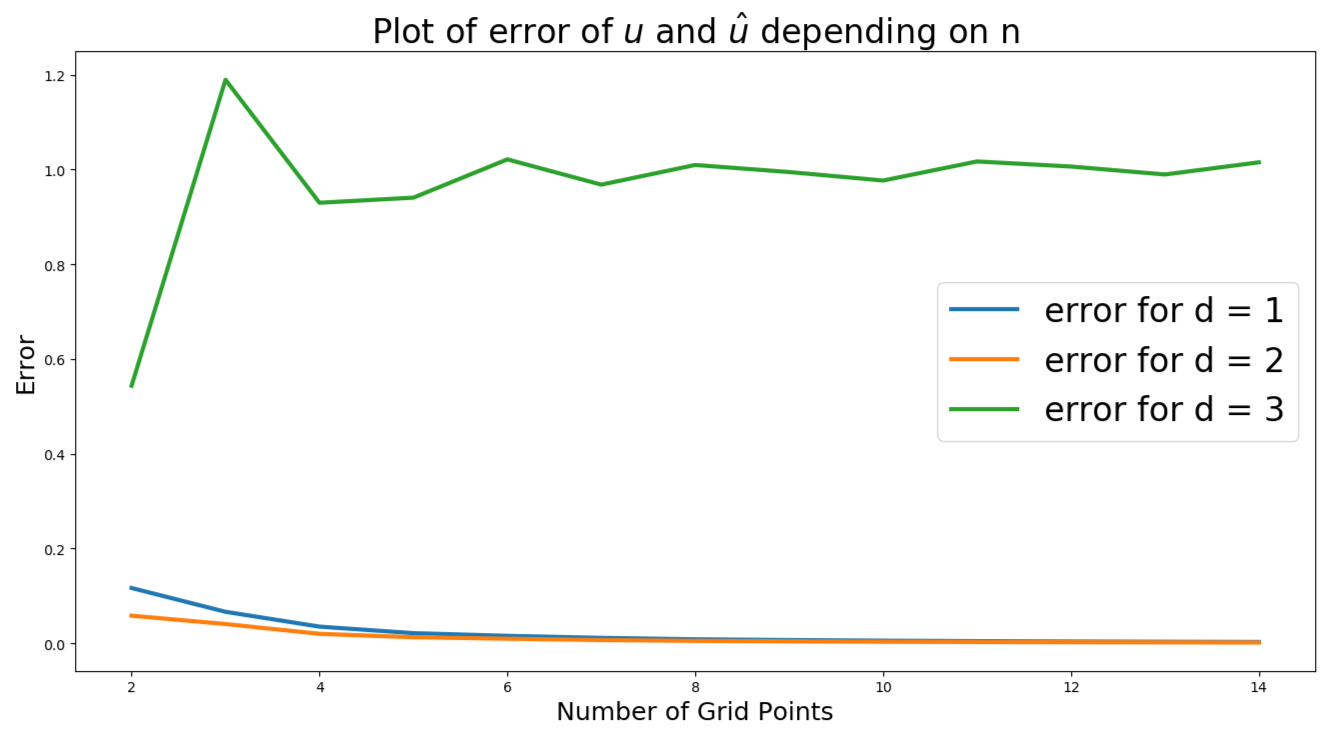
\includegraphics[width=\linewidth]{graphics/plot_error.png}
	\caption{Plot of the Error}
	\label{fig:plot_error}
\end{figure}
\bigskip

It turns out that the absolute error converges to a relativly small number. This is counter-intuitive at first because the condition number of the matrix \(A^{(d)}\) increases drastically for large \(N\) as seen on figure \ref{fig:cond_matrix}.

\begin{figure}[h]
	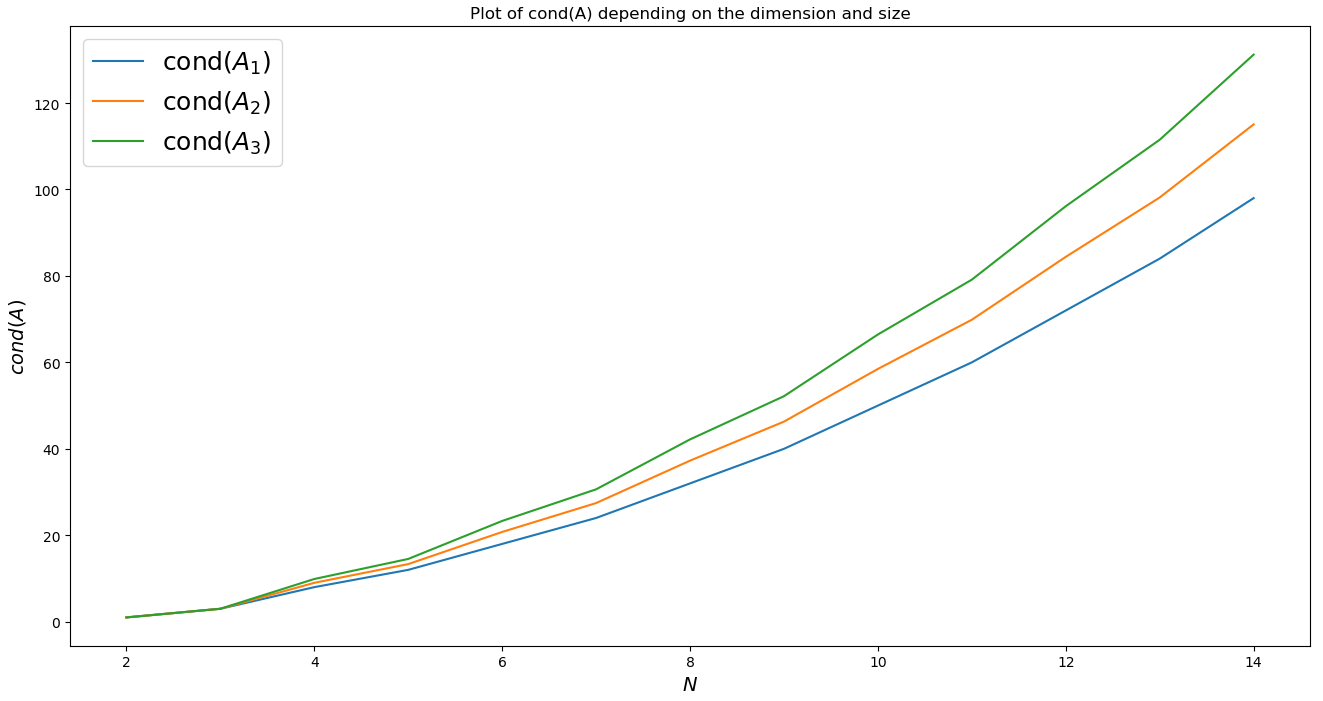
\includegraphics[width=\linewidth]{graphics/cond_matrix.png}
	\caption{Condition of the Matrix}
	\label{fig:cond_matrix}
\end{figure}
\bigskip

Why does the error of \(u\) and \(\hat{u}\) converge while the condition of \(A^{(d)}\) increases? To answer this question, we compare our results with the condition of the Hilbert Matrix which is well-known to be ill-conditioned (see figure \ref{fig:hilbert_condition}).

\begin{figure}[h]
	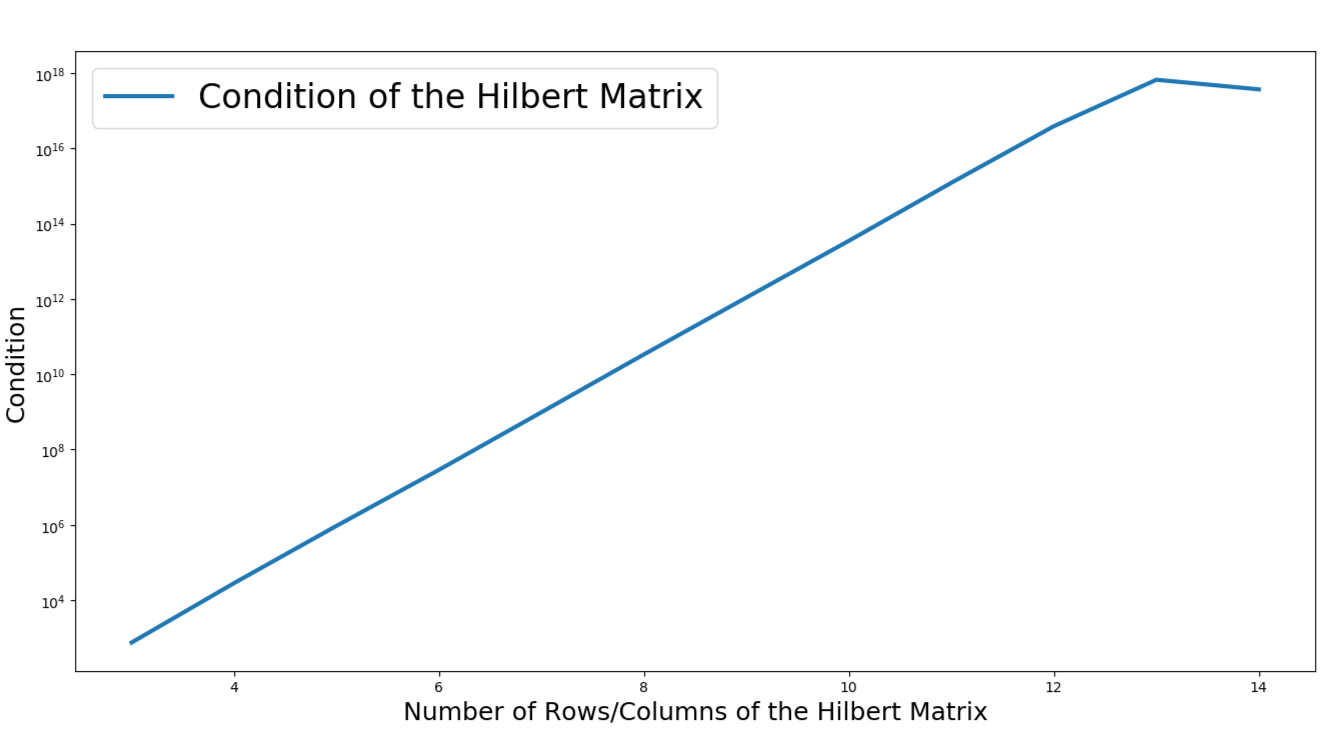
\includegraphics[width=\linewidth]{graphics/hilbert_condition.png}
	\caption{Condition of the Hilbert Matrix}
	\label{fig:hilbert_condition}
\end{figure}
\bigskip

As one can see, the condition of the Hilbert matrix is so large that the condition of \(A^{(d)}\) pales in comparison. In other words, \(A^{(d)}\) is relativly not ill-conditioned as one might assume at first. Furthermore, intuitively, the increase in number of grid points should make the approximation of the solution to the Poission's equation more accurate which is reflected on the convergence of the error plots.

\section{Sparsity of}

\begin{figure}[h]
	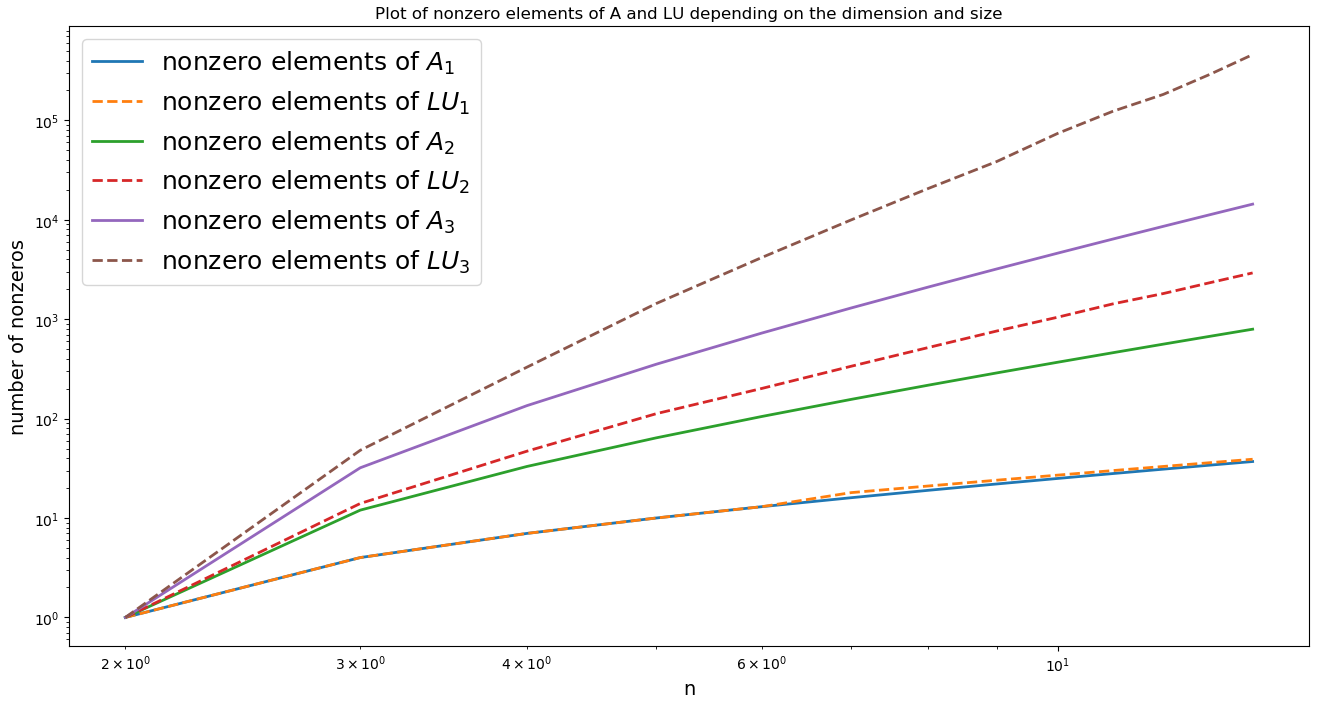
\includegraphics[width=\linewidth]{graphics/non_zero.png}
	\caption{Comparison of Nonzero Elements}
	\label{fig:boat1}
\end{figure}

\end{document}